\documentclass[article]{jss}
\usepackage[utf8]{inputenc}

\providecommand{\tightlist}{%
  \setlength{\itemsep}{0pt}\setlength{\parskip}{0pt}}

\author{
John Muschelli\\Department of Biostatistics, Johns Hopkins Bloomberg School of Public
Health
}
\title{ROC and AUC in R with a Single Binary Predictor}

\Plainauthor{John Muschelli}
\Plaintitle{ROC and AUC in R with a Single Binary Predictor}
\Shorttitle{Single Binary Predictor ROC}

\Abstract{
The abstract of the article.
}

\Keywords{roc, auc, area under the curve, \proglang{R}}
\Plainkeywords{roc, auc, area under the curve, R}

%% publication information
%% \Volume{50}
%% \Issue{9}
%% \Month{June}
%% \Year{2012}
%% \Submitdate{}
%% \Acceptdate{2012-06-04}

\Address{
    John Muschelli\\
  Department of Biostatistics, Johns Hopkins Bloomberg School of Public
  Health\\
  615 N Wolfe St Baltimore, MD 21205\\
  E-mail: \email{jmuschel@jhsph.edu}\\
  URL: \url{http://johnmuschelli}.\\~\\
  }

\usepackage{amsmath}

\begin{document}

\section{Introduction}\label{introduction}

This template demonstrates some of the basic latex you'll need to know
to create a JSS article.

\subsection{Code formatting}\label{code-formatting}

Don't use markdown, instead use the more precise latex commands:

\begin{itemize}
\tightlist
\item
  \proglang{Java}
\item
  \pkg{plyr}
\item
  \code{print("abc")}
\end{itemize}

\section{Simple Example}\label{simple-example}

\begin{CodeChunk}

\begin{CodeInput}
R> x = c(rep(0, 52), rep(1, 32),
R+       rep(0, 35), rep(1, 50))
R> y = c(rep(0, 84), rep(1, 85))
R> tab = table(x, y)
R> tab
\end{CodeInput}

\begin{CodeOutput}
   y
x    0  1
  0 52 35
  1 32 50
\end{CodeOutput}
\end{CodeChunk}

As there are only two outcomes for \(X\), we can expand the probability
using the law of total probability:

\begin{align}
P(X_{1} > X_{0}) &= P(X_{1} > X_{0} | X_{1} = 1) P(X_{1} = 1) \nonumber \\
&+ P(X_{1} > X_{0} | X_{1} = 0) P(X_{1} = 0) \label{eq:expand1} \\
&= P(X_{1} > X_{0} | X_{1} = 1) P(X_{1} = 1) \label{eq:expand}
\end{align}

where the second term of equation \eqref{eq:expand1} is equal to zero
because \(X_{0} \in \{0, 1\}\).

Here we see that the second term of equation \eqref{eq:expand} is the
sensitivity:

\begin{align*}
P(X_{1} = 1) &= P(X = 1 | Y = 1)\\
&= \frac{TP}{TP + FN} \\
&= \text{sensitivity}
\end{align*}

Here we show the first term of equation \eqref{eq:expand} is the
specificity:

\begin{align*}
P(X_{1} > X_{0} | X_{1} = 1) &= P(X_{1} > X_{0} | X_{1} = 1, X_{0} =1) P(X_{0} = 1) \\
&+ P(X_{1} > X_{0} | X_{1} = 1, X_{0} =0) P(X_{0} = 0) \\
&= P(X_{1} > X_{0} | X_{1} = 1, X_{0} =0) P(X_{0} = 0) \\
&= P(X_{0} = 0) \\
&= P(X = 0 | Y = 0)\\
&= \frac{TN}{TN + FP} \\
&= \text{specificity}
\end{align*}

Therefore, we combine these two to show that equation \eqref{eq:expand}
reduces to: \[
P(X_{1} > X_{0}) = \text{specificity} * \text{sensitivity}
\]

Therefore, the true AUC should be equal to:

\begin{CodeChunk}

\begin{CodeInput}
R> sens = tab[2,2] / sum(tab[,2])
R> spec = tab[1,1] / sum(tab[,1])
R> true_auc = sens * spec
R> print(true_auc)
\end{CodeInput}

\begin{CodeOutput}
[1] 0.3641457
\end{CodeOutput}
\end{CodeChunk}

\begin{CodeChunk}

\begin{CodeInput}
R> fpr = 1-spec
R> area_of_tri = 1/2 * sens * fpr
R> area_of_quad = sens * spec + 1/2 * spec * (1-sens)
R> auc = area_of_tri + area_of_quad
\end{CodeInput}
\end{CodeChunk}

We can also show that if we use a simple sampling method, we can
estimate this true AUC. Here, the function \code{est_auc} samples
10\^{}\{6\} random samples from \(X_{1}\) and \(X_{0}\), then calculates
\(\hat{P}(X_{1} > X_{0})\):

\begin{CodeChunk}

\begin{CodeInput}
R> est_auc = function(x, y) {
R+   x1 = x[y == 1]
R+   x0 = x[y == 0]
R+   n = 1000000
R+   c1 = sample(x1, size = n, replace = TRUE)
R+   c0 = sample(x0, size = n, replace = TRUE)
R+   mean(c1 > c0)
R+ }
R> sample_est_auc = est_auc(x, y)
R> sample_est_auc
\end{CodeInput}

\begin{CodeOutput}
[1] 0.364325
\end{CodeOutput}
\end{CodeChunk}

\section{Current Implementations}\label{current-implementations}

\subsection{R}\label{r}

\subsubsection{ROCR Package}\label{rocr-package}

The \pkg{ROCR} package is one of the most popular packages for doing ROC
analysis \cite{ROCR}. Using \code{prediction} and \code{performance}
functions, we see that the estimated AUC is much higher than the true
AUC:

\begin{CodeChunk}

\begin{CodeInput}
R> library(ROCR)
\end{CodeInput}

\begin{CodeOutput}
Loading required package: gplots
\end{CodeOutput}

\begin{CodeOutput}

Attaching package: 'gplots'
\end{CodeOutput}

\begin{CodeOutput}
The following object is masked from 'package:stats':

    lowess
\end{CodeOutput}

\begin{CodeInput}
R> pred = prediction(x, y)
R> auc_est = performance(pred, "auc")
R> auc_est@y.values[[1]]
\end{CodeInput}

\begin{CodeOutput}
[1] 0.6036415
\end{CodeOutput}
\end{CodeChunk}

Looking at the plot for the ROC curve in ROCR, we can see why this may
be:

\begin{CodeChunk}

\begin{CodeInput}
R> par(mfrow = c(1, 2))
R> perf = performance(pred, "tpr", "fpr")
R> plot(perf)
R> abline(a = 0, b = 1)
R> plot(perf, type = "s")
R> abline(a = 0, b = 1)
\end{CodeInput}
\end{CodeChunk}

\begin{CodeChunk}


\begin{center}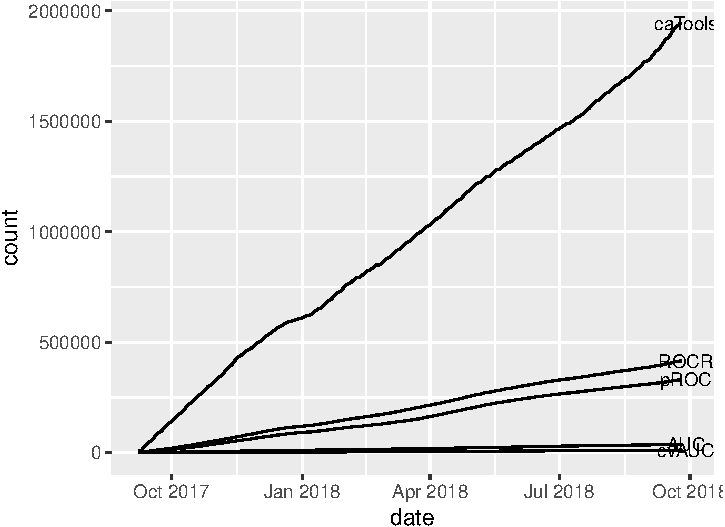
\includegraphics{index_files/figure-latex/unnamed-chunk-7-1} \end{center}

\end{CodeChunk}

Looking geometrically at the plot, we can see how

\begin{CodeChunk}

\begin{CodeInput}
R> fpr = 1 - spec
R> area_of_left_tri = 1/2 * sens * fpr
R> area_of_top_tri = 1/2 * spec * (1 - sens)
R> false_auc = area_of_left_tri + true_auc + area_of_top_tri
R> false_auc
\end{CodeInput}

\begin{CodeOutput}
[1] 0.6036415
\end{CodeOutput}
\end{CodeChunk}

\bibliography{binroc.bib}


\end{document}

